\documentclass{letter}
\usepackage{xcolor}
\usepackage{graphicx}
\usepackage{draftwatermark}
\usepackage{background}
\usepackage{hyperref}
\usepackage{blindtext}
\usepackage{multicol}
\usepackage{fancyhdr}
\usepackage{pgf-pie}
\usepackage{pgfplots}
\usepackage[a4paper, total={7in, 10in}]{geometry}
\usepackage{nopageno}
\setlength{\columnsep}{1cm}





\pgfplotsset{width=9cm,height=5cm,compat=1.7}  
\backgroundsetup{scale=0.5,opacity=0.5,contents=
\includegraphics{OI.png}}

\begin{document}
\begin{flushright}
\begin{scriptsize}
\textit{As per}
\textit{\textcolor{red}{UGC guidelines }}
\textit{an electronic bar code is provided to seure your paper}
\end{scriptsize}
\end{flushright}
\begin{multicols}{2}
\begin{flushleft}
\begin{scriptsize}
\textit{International Journal for Modern Trends in Science and Technology, }
 8(01): 124-129, 2022 Copyright © 2022 \newline International Journal for Modern Trends in Science and Technology International Journal for Modern Trends in Science and Technology  \newline ISSN: 2455-3778 online \newline DOI: \href{https://doi.org/10.46501/IJMTST0801022} {\textcolor{blue}{https://doi.org/10.46501/IJMTST0801022 }}\newline Available online at: \href { http://www.ijmtst.com/vol8issue01.html} {\textcolor{cyan}{ http://www.ijmtst.com/vol8issue01.html}}\newline \newline  

\includegraphics[width=.3\linewidth]{QR}\quad
\href{https://doi.org/10.46501/IJMTST0801022}{
\includegraphics[width=.2\linewidth]{check}}\quad
\href{http://www.ijmtst.com/vol7issue11.html}{
\includegraphics[width=.2\linewidth]{OI}}\quad
\end{scriptsize}
\end{flushleft}
\end{multicols}
\begin{LARGE}
\textbf {Automatic Hate Speech Detection on Social Media Text \newline using Machine Learning }\\ 
\end{LARGE} \newline 
\begin{small}\textbf{\begin{tabular}{l|c|r}J J C Prasad Yadav & Chimmani Aruna & N Srilatha \end{tabular}}
\end{small}
\begin{footnotesize}\\
\newline  Independent Researchers\newline  Corresponding Author Mail Id: \href{mailto:jagadishkrishnan0527@gmail.com}{\textcolor{blue}{jagadishkrishnan0527@gmail.com}} ,\href{mailto: arunachimmani@gmail.com}{\textcolor{blue}{ arunachimmani@gmail.com}} , \href{mailto:srilathancse@gmail.com}{\textcolor{blue}{srilathancse@gmail.com }}   \\  
\end{footnotesize}
\begin{small}\newline 
\textbf{To Cite this Article}\newline
J J C Prasad Yadav, Chimmani Aruna and N Srilatha. Automatic Hate Speech Detection on Social Media Text using 
Machine Learning.\textit{ International Journal for Modern Trends in Science and Technology }2022, \textit{8} pp. 124-129.\newline
\href{https://doi.org/10.46501/IJMTST0801022}{\textcolor{blue}{https://doi.org/10.46501/IJMTST0801022}}\newline   \\ 
\textbf{Article Info}\newline
Received: 16 November 2021; Accepted: 01 January 2022; Published: 06 January 2022
\end{small}\newline
\noindent\rule{7in}{2pt}

\colorbox{black}{\textcolor{white}{ABSTRACT}}\\
\begin{footnotesize}
\textbf{\textit {The increasing use of social media and information sharing has given major benefits to humanity. However, this has also given 
rise to a variety of challenges including the spreading and sharing of hate speech messages. Hate speech is one type of harmful 
online content which directly attacks or promotes hate towards a group, or an individual member based on their actual or 
perceived aspects of identity, such as ethnicity, religion, and sexual orientation. With online hate speech on the rise, its automatic 
detection as a natural language processing task is gaining increasing interest. In our work, we included pre-processing (stop word 
removal and stemming) and multiple classifiers for performance evaluation. The results we obtained were satisfactory.\\  \\
Keywords: social media, Hate speech, Abusive language, machine learning, natural language processing and Text classification.}}
\end{footnotesize}
\noindent\rule{7in}{2pt}
\begin{multicols}{2}
\begin{large}\textbf{1.INTRODUCTION}\end{large}\\ \begin{normalsize}
The debate around the regulation of hate speech is still 
ongoing [1]. It is still not clear whether the best response 
to it is through legal measures, or other methods (such 
as counter-speech and education [2]). Regardless of the 
means of countering it, the evident harm of hate speech 
[3] makes its detection crucial. Both the volume of 
content generated online, particularly in social media, 
and the psychological burden of manual moderation [4] 
supports the need for the automatic detection of 
offensive and hateful content.
Online hate, described as abusive language [5], 
aggression [6], cyberbullying [7, 8], hatefulness [9], 
insults [10], personal attacks [11], provocation [12], 
racism [13], sexism [14], threats [15], or toxicity [16], has 
been identified as a major threat on online social media 
platforms. Pew Research Centre [17] reports that among 
4248 adults in the United States, 41\% have personally \\ \\
experienced harassing behaviour online, whereas 66\% 
witnessed harassment directed towards others. Around 
22\% of adults have experienced
offensive name-calling, purposeful embarrassment 
(22\%), physical threats (10\%), and sexual harassment 
(6\%), among other types of harassment. Social media 
platforms are the most prominent grounds for such 
toxic behaviour. Even though they often provide ways 
of flagging offensive and hateful content, only 17\% of all 
adults have flagged harassing conversation, whereas 
only 12\% of adults have reported someone for such acts 
[17]. 
In the following paragraphs, we better tried to 
differentiate Hate speech, offensive language, and 
abusive language. Although different types of abusive 
and offensive language are closely related, there are 
important distinctions to note. Offensive language and 
abusive language are both used as umbrella terms for
\end{normalsize}
\end{multicols}

\pagestyle{fancy}
\lfoot{ {\noindent\rule{7in}{2pt}} \\ \textbf{ \thepage \hspace{0.4cm}  {\textcolor{red}{International Journal for Modern Trends in Science and Technology}}}}





\begin{multicols}{2}
\begin{normalsize}{harmful content in the context of automatic detection 
studies. However, while ``strongly impolite, rude'' and 
possible use of profanity are seen in the definitions of 
both, abusive language has a strong component of 
intentionality. Thus, offensive language has a broader 
scope, and hate speech falls in both categories. Because 
of its definition mentioned above, hate speech is also 
different from other subtypes of offensive language. For 
example, personal attacks are characterised by being 
directed at an individual, which is not necessarily 
motivated by the target's identity. Hate speech is also 
different from cyberbullying which is carried out 
repeatedly and over time against vulnerable victims 
that cannot defend themselves. This paper focuses on 
hate speech and hate speech datasets, although studies 
that cover both hate speech and other offensive 
language are also mentioned.}
\end{normalsize}\\ \\ \\ \\
\begin{normalsize}\textbf{2.RELATED WORK}\end{normalsize}\\  \\ \\
\begin{normalsize}{Abusive messages in social media is a complex 
phenomenon with a broad range of overlapping modes 
and goals [18]. Cyberbullying and hate speech are 
typical examples of abusive languages that researchers 
have put more interest in the past few decades due to 
their negative impacts in our societies. Several research 
have been conducted to automatically detect these 
undesirable messages among other messages in social 
media. The automatic detection of hate speech using 
machine learning approaches is relatively new, and 
there are very limited review papers on techniques for 
automatic hate speech detection [19]. \\ \\
The recent and related survey papers available on 
review of hate speech detection methods during this 
research work were few. The following were the 
available traditional literature review related to 
automatic detection of hate speech using MLA: [20], ML 
algorithms have contributed immensely to hate speech 
detection and SM content analysis generally [21]. 
Offensive comments such as HS and cyberbullying are 
the most researched areas in NLP in the past few 
decades [22].\\ \\

ML algorithms have been of great help in this 
direction in terms of SM data analysis for the 
identification and classification of offensive comments 
[23]. The advances in ML algorithms research have 
made significant impacts in many \_elds of endeavour 
which led to some important tools and models for
analysing a large amount of data in real-world 
problems like SMNs content analysis [24]. In this survey 
conducted by [25], the authors presented a brief review 
on eight hate speech detection techniques and 
approaches. These eight techniques include TF-IDF, 
dictionaries, N-gram, sentiment analyses, 
template-based approach, part of speech, Bag of the 
word, and rule-based approach. The limitation of the 
review is that techniques such as deep learning and 
ensemble approach were not considered in their work. 
In [19], the authors offered a brief, and critical analysis 
of the areas of automated hate speech detection in 
natural language processing. The authors also analysed 
the features for hate speech detection in literature which 
includes simple surface features, word generalization, 
sentiment analysis, lexical resources, linguistic features, 
knowledge-based features, meta-information, and 
multimodal information. The limitation of these two 
reviews is that techniques such as deep learning and 
ensemble approach are not considered in their work. 
The most significant step in text classification pipeline is 
selection of the best classifier [26]. Therefore, the need to 
review all techniques is of essence. We intent to make 
this selection phase easier for researchers by reviewing 
more algorithms than the previous review work has 
covered. In this case, we reviewed techniques like deep 
learning, ensemble learning among others that have 
been employed for the automatic detection of hate 
speech in social media. Posters of hate speeches usually 
attack their targets using the following attributes: 
Religion, Race, political affiliation, gender, marital 
status, ethnicity, health status, disability, and 
nationality [27]. The following diagram shows the 
worldwide most popular social networks as of October 
2021[28], ranked by number of active users (in millions).}
\end{normalsize}\\ \\

\begin{tiny}
\begin{center}
Most popular social networks worldwide(as of 
October 2021), ranked by number of active users (in 
millions)
\end{center}
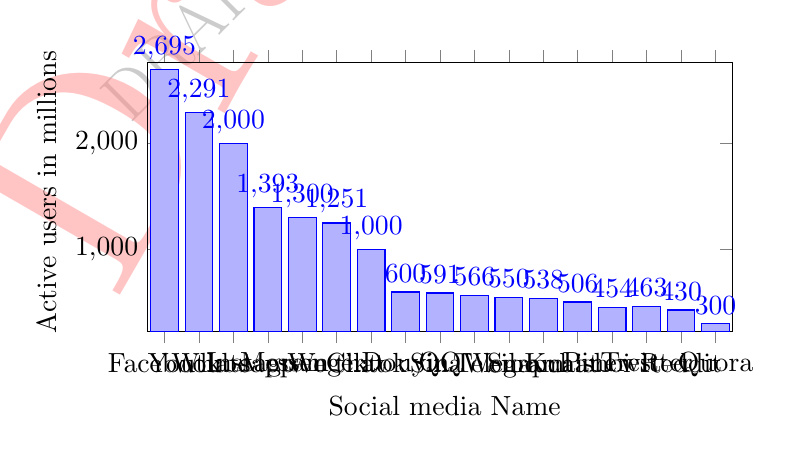
\begin{tikzpicture}  
  \begin{axis}  
[  
    ybar,  
    enlargelimits=0.03,  
    ylabel={\ Active users in millions},
    xlabel={\ Social media Name},  
    symbolic x coords={Facebook,Youtube,Whatsapp,Instagram,Messenger,WeChat,tiktok,Douyin,QQ,SinaWeibo,Telegram,Snapchat,Kuaishoi,Pinerest,Twitter,Reddit,Quora}, 
    xtick=data,  
     nodes near coords, 
    nodes near coords align={vertical},  
    ]  
\addplot coordinates { (Facebook,2695)(Youtube,2291)(Whatsapp,2000)(Instagram,1393)(Messenger,1300)(WeChat,1251)(tiktok,1000)(Douyin,600)(QQ,591)(SinaWeibo,566)(Telegram,550)(Snapchat,538)(Kuaishoi,506)(Pinerest,454)(Twitter,463)(Reddit,430)(Quora,300)};  
\end{axis}  
\end{tikzpicture} 
\end{tiny}


\begin{normalsize}{Fig.1: Most popular social networks worldwide (as of 
October 2021), ranked by number of active users (in 
millions)}\end{normalsize}
\end{multicols}


\newpage
\begin{multicols}{2}
\begin{large}{\textbf{3.Challenges of Detecting Hateful and Offensive
Speech}}\end{large} \\ \\ 
There are many layers to the difficulty of automatically 
detecting hateful and/or offensive speech, particularly 
in social media. Some of these difficulties being closely 
related to the shortcomings of keyword-based 
approaches. For one, words can be obfuscated in many 
ways, both in an intentional attempt to avoid automatic 
content moderation, or because of the use of social 
media for communication (consider, for example the 
tendency in some posts to replace letters with similar 
looking numbers, e.g., “E”s with 3s, or “l”s with 1s, and 
so on). Furthermore, there are many expressions that 
are not inherently offensive, however they can be so in 
the right context. But even in the case of slurs, not only 
different slurs hold a different degree of offense, but the 
offense can also also vary based on different time (as 
previously innocuous words may become slurs in time), 
as well as different use of the same word, different 
users, and different audience members. One example of 
this is the difference in the use of slurs by in-group 
speakers, and out-group speakers. This factor, when 
disregarded can contribute to the bias in hate speech 
detection corpora (against African
Americans, and more specifically, against African 
American men), and in turn, the bias in hate speech 
detection (a strong argument for the transparency and 
explainability of hate speech detection models). \\ 
One recommendation to mitigate bias is explicitly 
preparing annotators for it. This leads to another 
difficulty, namely the availability (or lack thereof) of 
reliably annotated data. A factor that contributes to this 
problem is that there is no universally accepted 
definition of hate speech (a statement many 
publications would agree on, let alone one that is 
productive. One can point at a United Nations report for 
definition, we would however argue that it does not 
satisfy the criteria of being a universally accepted 
productive definition on several accounts. For one, the 
recommendations in said document are not legally 
binding, thus their implementation in all member 
countries is not a given. Furthermore, the 
recommendation here is only to “draw [...] from the 
guidance and definitions”, not to apply them as it is, 
thus even if the recommendations were binding, or all 
member countries would decide by their own volition 
to accept them, different countries could still arrive at
different definitions implemented in their domestic 
legal frameworks. Moreover, even if the definitions 
were used “as is”, the question remains whether they 
would be applicable for large scale data annotation, 
considering the contextual nature of their terms (“First, 
one should realize that the question of distinguishing 
those forms of expression that should be defined as 
incitement to hatred and thus prohibited is contextual 
and the individual circumstances and the individual 
circumstances of each case, such as local conditions, 
history, cultural and political tensions, must be 
considered”), and the complexity of definitions that 
could necessitate annotators having a background in 
law.\\
One benefit of a universally agreed upon productive 
definition for hate speech could be important for more 
reliable annotation, with higher inter-annotator 
agreement. For example, the 2019 HASOC hate speech 
and offensive content evaluation task had an interrater 
agreement rate that is between 69 and 77 percent for 
different task, even though “many texts recommend 
80% agreement as the minimum acceptable interrater 
agreement” [30]. According to Mandl et al. [31] (the 
organizers of the 2019 HASOC hate speech and 
offensive content evaluation task), one difficulty in 
annotation (an issue that may have contributed to the 
low interrater agreements) was the use of language 
registers, such as youth talk. The difficulty of annotating 
youth talk is exemplified by the annotation of some 
example tweets (see Table 1) where the name of India’s 
prime minister (Narendra Modi, or Modi Ji) was used in 
various pop-cultural references (or” memes”). The first 
being a paraphrase of the chorus(“Never gonna give you 
up // Never gonna let you down // Never gonna run around 
and desert you...”) from the 1987 Rick Astley hit, Never 
Gonna Give You Up (that gained a considerable 
reputation in recent years, due to its use in the 
phenomenon called” rickrolling”). The second being a 
reference to a popular beverage that is well known for 
the company’s secrecy regarding its recipe. While the 
third referencing a much-quoted part of a recent movie, 
and the last one making a reference to a 1998 song from 
Baha Man (Who let the dogs out). Despite the similar 
nature of the tweets (particularly the last three tweets, 
as all three of them allude to Modi Ji knowing 
something that in general considered impenetrable - as 
mentioned before, the ingredients of Coca Cola are
\end{multicols}

\newpage
\begin{multicols}{2}
considered a well-kept secret; part of the comedic effect 
of Drax the destroyer asking the question “Why is 
Gamorra” is derived from the fact that this question 
itself is considered unanswerable; and not only the song 
does not answer the question, who let the dogs out, but 
two of the artists contributing to the song also refused to 
do so in recent interviews), however, two were labelled 
as hateful or offensive, while the other two were not. 
Here, it is important to note that our argument is not 
that all these tweets should be annotated as hate speech, 
but rather that these tweets should have a uniform 
annotation. And in our opinion, given the innocuous 
nature of the references, they would be annotated as not 
hateful, given an annotator who is aware of the cultural 
context.\\
Another example that may result from the annotation 
of hateful or offensive speech being subjective is that of 
the labelling of tweets containing the word fuck 
(subsequently referred to as the “f-word”). Particularly, 
the difference in labelling between the case when the 
word is used as part of a hashtag, as opposed to when it 
is used outside of a hashtag. 

\begin{footnotesize}
\begin{center}
{\textbf{Table 1 Tweets where the name of the Indian prime minister is used 
in pop-cultural references, and their annotations}}
\begin{tabular}{|l|c|}
\hline
\textbf{Tweet} & \textbf{Annotation}\\[0.5ex]
\hline
Modi Ji will never give you up & Not hateful/offensive\\
Modi ji will &   \\
never give you down & hateful/offensive\\
Modi Ji knows Coca Cola’s & Hateful/offensive\\
secret ingredient Not & Hateful/offensive\\
Modi Ji knows why is Gamora &  \\
Modi Ji knows who let the dogs out &  \\
\hline
\end{tabular}
\end{center}
\end{footnotesize}
\textbf{Our work:}\\\\
We have used the most popular dataset [29] for the 
experimental evaluation. The following diagrams better 
describes the classes distribution in the dataset.\\ \\
\begin{scriptsize}
\begin{center}
HateSpeechData dataset classes distribution
\end{center}
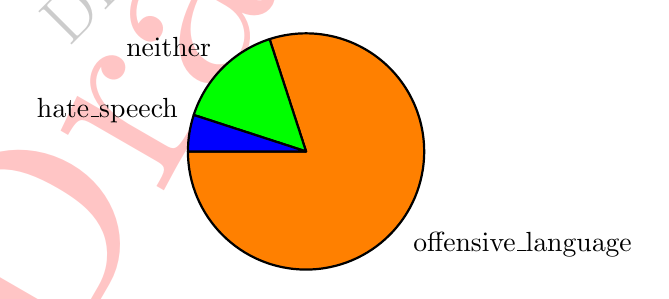
\begin{tikzpicture}
\pie [rotate = 180,radius=1.5,color = {orange,green,blue},hide number]
    {80/ offensive\_language,
     15/neither, 5/hate\_speech}
\end{tikzpicture}
\end{scriptsize}\\
Fig.2: HateSpeechData dataset classes distribution\\ \\ \\ \\ \\ \\ \\ \\ \\ \\ \\ \\ \\
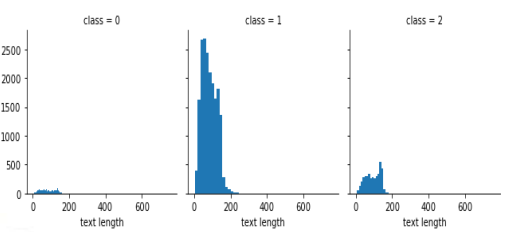
\includegraphics[width=1\linewidth]{aa}\\ 
\begin{center}Fig.3: visualization of dataset classes data using 
histograms
\end{center}
We removed punctuations and made the dataset text 
case insensitive. We applied pre-processing techniques 
like stop word removal and stemming. We have 
visualized the words which commonly present in 
different classes and in the dataset as follows.

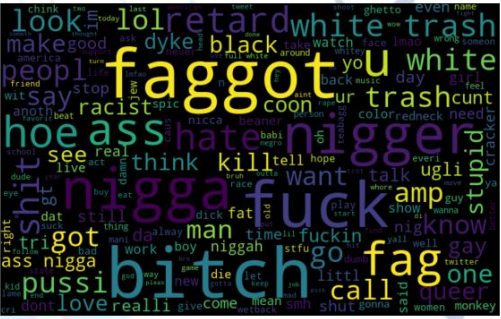
\includegraphics[width=1\linewidth]{bb}\\ 
Fig. 4(a) Most used words of hatred class\\ \\
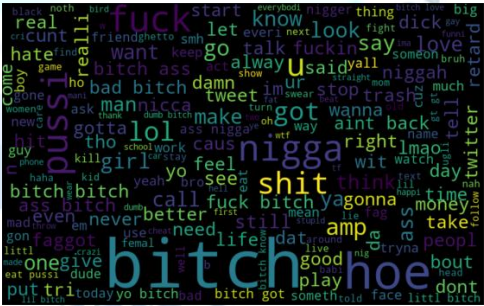
\includegraphics[width=1\linewidth]{cc}\\ \\ 
Fig. 4(b) Most used words of offensive class



\newpage

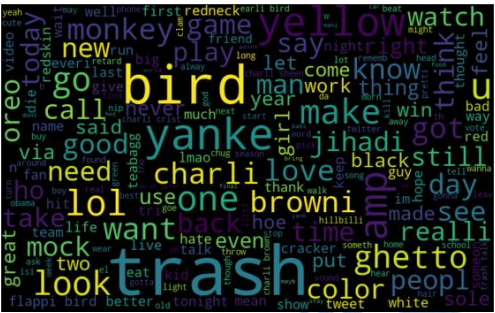
\includegraphics[width=1\linewidth]{dd}\\ \\
Fig. 4(c) Most used words in the class 2 (neither hatred 
nor offensive) \\ \\
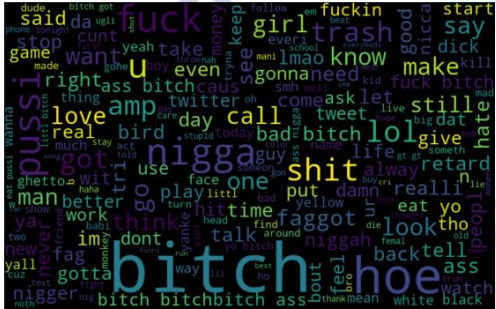
\includegraphics[width=1\linewidth]{ee}\\  \\
Fig. 4(d) Most used words in entire data set\\ \\
We have used TFIDF feature weighting technique to rep
resent the dataset in bag of words model. The feature ve
ctor resulted is a big sparse matrix of size 24783x6441.W
e have used four different classifiers for classification. L
ogistic Regression, Random Forest, Naive Bayes and SV
M. \\ \\


\begin{tiny}
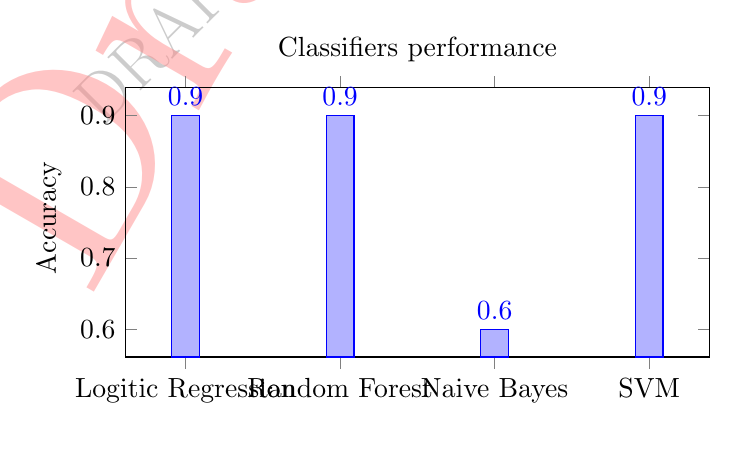
\begin{tikzpicture}   
\begin{axis}  
[  
title=Classifiers performance,
    ybar,  
    enlargelimits=0.13,  
    ylabel={\ Accuracy},
    xlabel={\ },  
    symbolic x coords={Logitic Regression,Random Forest,Naive Bayes,SVM}, 
    xtick=data,  
     nodes near coords, 
    nodes near coords align={vertical},  
    ]  
\addplot coordinates { (Logitic Regression,0.9)(Random Forest,0.9)(Naive Bayes,0.6)(SVM,0.9)};  
\end{axis}  
\end{tikzpicture} 
\end{tiny}
\begin{center}
Fig.5: Classifiers performance 
\end{center}
\begin{large}{\textbf{4. RESULTS AND DISCUSSION}}\end{large} \\ \\   \newline \newline
The results clearly show that differentiating hate 
speech and offensive language is a challenging task. The 
language or text used in expressing hate or abusing\\ 
someone in online is incomplete. In other words, we can 
say that some words used in expressing hate or during 
abuse does not belonging to any natural language. 
Emojis and image expression processing techniques 
may also work well in this area. It also indicates the 
benefits of using the proposed features and provides a 
valuable resource for detecting the problem of toxic 
language on twitter. Fig. 4(a), (b), (c) and (d) visualizes 
the important features of the label or dataset as 
described in the figure names. These figures better 
describe the words distribution in categories as well as 
in the dataset. Although a detailed analysis of the 
features as well as errors could lead to more robust 
feature extraction methods and help us in solving the 
existing challenges in this field. Except Naïve Bayes, 
remaining all classifiers performed predominantly well 
as shown in Fig.5.\\ \\
\begin{large}{\textbf{5.CONCLUSION}}\end{large} \\ \\ 
Generalisability is a complex problem concerning 
every aspect of hate speech detection \_dataset building, 
model training and evaluation, and application. Thus, 
obstacles to generalisable hate speech detection are 
largely intertwined. In the ``obstacles'' section above, we 
analysed the problem of generalisability and discussed 
existing research, organised by obstacles and their 
causes. Here, we suggest what can practically be done 
moving forward, from the specific perspectives of 
dataset and models, as well as other general challenges. 
These suggestions vary by problem complexity and 
generality. Nonetheless, they are all, in our opinion, 
critical things to keep in mind for any researcher 
working on hate speech detection to evaluate and 
improve generalisability.\\ \\ \\ \\  
\begin{small}{\textbf{REFERENCES}}\\ \\
\end{small}
\begin{scriptsize}{[1] Barendt, E.: What is the harm of hate speech? Ethic theory. Moral 
Pract. 22, 2019. https ://doi.org/10.1007/s1067 7-019-10002 -0. \newline \newline
[2] Brown A. What is so special about online (as compared to offline) 
hate speech? Ethnicities. 2018;18(3):297–326. https 
://doi.org/10.1177/14687 96817 709846. \newline \newline
[3] Müller K, Schwarz C. Fanning the flames of hate: social media 
and hate crime. SSRN Electronic Journal; 2017.https 
://doi.org/10.2139/ssrn.3082972. \newline \newline
[4] https ://www.thegu ardia n.com/techn ology /2019/sep/17/revea 
led-catastrophic-effects-workingfacebook-moderator. \newline \newline
[5] Castelle M. The linguistic ideologies of deep abusive language 
classification. In: Proceedings of the 2nd workshop on abusive 
language online (ALW2), Brussels; 2018. P. 160–70}


\newpage

[6] Kumar S, et al. Community interaction and conflict on the web. 
In: Proceedings of the 2018 world wide web conference on world 
wide web; 2018. P. 933–43. \newline \newline
[7] Hosseinmardi H et al (2015) Analyzing labeled cyberbullying 
incidents on the instagram social network. Soc Inf 2015:49–66.
[8] Wachs S et al (2019) Understanding the overlap between 
cyberbullying and cyberhate perpetration: moderating effects of 
toxic online disinhibition. Crim Behav Mental Health 
29(3):179–188.\newline \newline
[9] Salminen J, et al. Anatomy of online hate: developing a 
taxonomy and machine learning models for identifying and 
classifying hate in online news media. In: Proceedings of the 
international AAAI conference on web and social media 
(ICWSM 2018), San Francisco; 2018.\newline \newline
[10] Sood SO et al (2012) Automatic identification of personal insults 
on social news sites. J Am Soc Inform Sci Technol 63(2):270–285.
[11] Wulczyn E, et al. Ex Machina: personal attacks seen at scale. In: 
Proceedings of the 26th international conference on world wide 
web, Geneva; 2017. P. 1391–9.\newline \newline
[12] Mkono M (2018) ‘Troll alert!’: provocation and harassment in 
tourism and hospitality social media. Curr Issues Tour 
21(7):791–804.\newline \newline
[13] Waseem Z. Are you a racist or am i seeing things? Annotator 
influence on hate speech detection on twitter. In: Proceedings of 
the first workshop on NLP and computational social science; 
2016. P. 138–42.\newline \newline
[14] Chatzakou D, et al. Measuring \#GamerGate: A tale of hate, 
sexism, and bullying. In: Proceedings of the 26th international 
conference on world wide web companion, Geneva; 2017. P. 
1285–90.\newline \newline
[15] Willard NE (2007) Cyberbullying and cyberthreats: Responding 
to the challenge of online social aggression, threats, and distress. 
research press, Champaign.\newline \newline
[16] Märtens M, et al. Toxicity detection in multiplayer online games. 
In: Proceedings of the 2015 international workshop on network 
and systems support for games, Piscataway; 2015. P. 5:1–5:6.\newline \newline
[17] Pew Research Center 2017. Online Harassment 2017.\newline \newline
[18] R. Alshalan and H. Al-Khalifa, ``A deep learning approach for 
automatic hate speech detection in the Saudi Twittersphere,'' 
Appl. Sci., vol. 10, no. 23, pp. 1\_16, 2020.\newline \newline
[19] A. Al-Hassan and H. Al-Dossari, ``Detection of hate speech in
social networks: A survey on multilingual corpus,'' in Proc. 
Comput. Sci. Inf.Technol. (CS IT), Feb. 2019, pp. 83\_100.\newline \newline
[20] A. Schmidt and M. Wiegand, ``A survey on hate speech detection 
using natural language processing,'' in Proc. 5th Int. Workshop 
Natural Lang.Process. Social Media, 2017, pp. 1\_10.\newline \newline
[21] M. A. Al-Garadi, M. R. Hussain, N. Khan, G. Murtaza, H. F. 
Nweke, I. Ali, G. Mujtaba, H. Chiroma, H. A. Khattak, and A. 
Gani,``Predicting cyberbullying on social media in the big data 
era using machine learning algorithms: Reviewof literature and 
open challenges,'' IEEE Access, vol. 7,pp. 70701\_70718, 2019.\newline \newline
[22] Rodriguez, C. Argueta, and Y.-L. Chen, ``Automatic detection of 
hate speech on Facebook using sentiment and emotion analysis,'' 
in Proc. Int. Conf. Artif. Intell. Inf. Commun. (ICAIIC), Feb. 2019, 
pp. 169\_174.\newline \newline
[23] G. Weir, K. Owoeye, A. Oberacker, and H. Alshahrani, 
``Cloud-based textual analysis as a basis for document
classi\_cation,'' in Proc. Int. Conf. High Perform. Comput. Simul. 
(HPCS), Jul. 2018, pp. 629\_633.\newline \newline
[24] J. Cheng, C. Danescu-Niculescu-Mizil, and J. Leskovec, 
``Antisocial behavior in online discussion communities,'' in Proc. 
9th Int. Conf. Web Soc. Media (ICWSM), 2015, pp. 61\_70, 2015.\newline \newline
[25] A. Alrehili, ``Automatic hate speech detection on social media: A 
brief survey,'' in Proc. IEEE/ACS 16th Int. Conf. Comput. Syst. 
Appl. (AICCSA), Nov. 2019, pp. 1\_6.\newline \newline
[26] K. Kowsari, K. J. Meimandi, M. Heidarysafa, S. Mendu, L. 
Barnes, and D. Brown, ``Text classi\_cation algorithms:Asurvey,'' 
Information, vol. 10, no. 4, pp. 1\_68, 2019.\newline \newline
[27] T. Granskogen and J. A. Gulla, ``Fake news detection: Network 
data from social media used to predict fakes,'' in Proc. CEUR 
Workshop, vol. 2041, no. 1, 2017, pp. 59\_66.\newline \newline
[28] https://www.statista.com/statistics/272014/global-social-network
s-ranked-by-number-of-users/\newline \newline
[29] Davidson et al., “ Automated Hate Speech Detection and the 
Problem of Offensive Language”, Proceedings of the 11th 
International AAAI Conference on Web and Social Media, 2017.\newline \newline
[30] McHugh M. Interrater reliability: the kappa statistic. Biochemia 
medica : časopis Hrvatskoga društva medicinskih biokemičara / 
HDMB. 2012;22:276–82.\newline \newline
[31] Mandl T, Modha S, Patel D, Dave M, Mandlia C, Patel A. 
Overview of the HASOC track at FIRE 2019: Hate Speech and 
Offensive Content Identification in Indo-European Languages). 
In: Proceedings of the 11th annual meeting of the Forum for 
Information Retrieval Evaluation; 2019.


\end{scriptsize}
\end{multicols}
\end{document}


